\documentclass[twoside, 11pt]{article}

\usepackage[sc]{mathpazo} % Use the Palatino font
\usepackage{textcomp}
\usepackage[T1]{fontenc} % Use 8-bit encoding that has 256 glyphs
\linespread{1.05} % Line spacing - Palatino needs more space between lines
\usepackage{microtype} % Slightly tweak font spacing for aesthetics

\usepackage[english]{babel} % Language hyphenation and typographical rules

\usepackage[hmarginratio=1:1,top=32mm,columnsep=20pt]{geometry} % Document margins
\usepackage[hang, small,labelfont=bf,up,textfont=it,up]{caption} % Custom captions under/above floats in tables or figures
\usepackage{booktabs} % Horizontal rules in tables

\usepackage{lettrine} % The lettrine is the first enlarged letter at the beginning of the text

\usepackage{enumitem} % Customized lists
\setlist[itemize]{noitemsep} % Make itemize lists more compact

\usepackage{abstract} % Allows abstract customization
\renewcommand{\abstractnamefont}{\normalfont\bfseries} % Set the "Abstract" text to bold
\renewcommand{\abstracttextfont}{\normalfont\small\itshape} % Set the abstract itself to small italic text

\usepackage{titlesec} % Allows customization of titles
\renewcommand\thesection{\Roman{section}} % Roman numerals for the sections
\renewcommand\thesubsection{\arabic{subsection}} % roman numerals for subsections
\titleformat{\section}[block]{\large\scshape\centering}{\thesection.}{1em}{} % Change the look of the section titles
\titleformat{\subsection}[block]{\large}{\thesubsection.}{1em}{} % Change the look of the section titles

\usepackage{fancyhdr} % Headers and footers
\pagestyle{fancy} % All pages have headers and footers
\fancyhead{} % Blank out the default header
\fancyfoot{} % Blank out the default footer
\fancyhead[C]{F70 - Mechanik und Vakuum $\bullet$ April 2018 $\bullet$ Thimo Preis \& Tobias Abele} % Custom header text
\fancyfoot[RO,LE]{\thepage} % Custom footer text

\usepackage{titling} % Customizing the title section

\usepackage{hyperref} % For hyperlinks in the PDF
\hypersetup{bookmarks=true,bookmarksopen=true}

%----------------------------------------------------------------------------------------
%\usepackage[backend=biber,
%style=numeric,
%bibencoding=ascii
%]{biblatex}
%\addbibresource{Bibliography.bib}
%	TITLE SECTION
%----------------------------------------------------------------------------------------

\setlength{\droptitle}{-4\baselineskip} % Move the title up

\pretitle{\begin{center}\Huge\bfseries} % Article title formatting
	\posttitle{\end{center}} % Article title closing formatting
\title{F70: Mechanik und Vakuum} % Article title
\author{%
	\textsc{Thimo Preis and Tobias Abele}\thanks{Betreut von ...} \\[1ex] % Your name
	\normalsize Ruprecht-Karls-Universität Heidelberg
	%\normalsize 
}
\date{16.04-20.04.2018}


\usepackage{physics}
\usepackage{amsmath}
\usepackage{amssymb}
\usepackage{wasysym}
\usepackage{floatflt}

\usepackage{graphicx}
\usepackage{tikz}
\usetikzlibrary{shapes,calc,intersections,arrows.meta}
\usetikzlibrary{patterns,circuits.ee.IEC}
\usepackage{pgfplots}
\pgfplotsset{compat=1.15}

	

\begin{document}
	

	\maketitle
	
		\begin{abstract}
		\noindent
	\label{Abstract}
\noindent
The goal of this experiment is to do research on the characteristics of the muon. In detail we want to determine the lifetime and polarization of cosmic muons, which would also prove parity-violation in the weak interaction. For all our measurements we have six layers of scintillators with metal in between. Furthermore we can add a homogeneous magnetic field so that the muon will do a larmor-precession around the direction of the field. This makes it possible to determine the larmor-frequency, the magnetic moment of the muon and the polarization. The evaluation was done with ROOT.

\begin{table}[h]
	\centering
\begin{tabular}{lll}
	\toprule
	Physical Property & Abbreviation & Measured Value \\
	\midrule
	Lifetime & $\tau _{0}$ & $\left(2229 \pm 40.6_{stat} \pm 24.36_{sys} \right)\mathrm{ns}$\\
	
	Capture Lifetime & $\tau _{C}$ & $\left(961.1 \pm 110.8_{stat} \pm 79.11_{sys} \right) \mathrm{ns}$\\
	
	Coupling Constant& $G_F$&$\left(1.155 \pm 0.035 \right)\times 10^{-11} \mathrm{MeV} ^{-2}$\\
	
	Larmor Frequency & $\omega _{Larmor}$ &$\left(3.342 \pm 0.028_{stat} \pm 0.041_{sys}\right) \mathrm{MHz}$\\
	
	Magnetic Moment & $\mu _{mu}$ & $\left(2.75 \pm 0.04\right)\times 10^{-7} \mathrm{eV T^{-1}}$\\
	
	Polarization & P & $\left(0.23 \pm 0.11_{stat} \pm 0.03_{sys}\right)$\\
	\bottomrule
\end{tabular}
\caption{Measured Values}
\label{tab:1.Tab}
\end{table}
\end{abstract}
	\section{Physikalische Grundlagen}
\subsection{Entstehung und Zerfall von Myonen}
Im Experiment werden Myonen betrachet, die durch kosmische Höhenstrahlung erzeugt werden. Diese besteht überwiegend aus hochenergetischen Protonen, die dann in der oberen Atmosphäre mit Molekülen wechselwirken. Dabei finden folgende Reaktionen statt:
\begin{align}
	&p+p \rightarrow p+n+\pi ^{+} \\
	&p+n \rightarrow p+p+\pi ^{-}\\
	&p+p \rightarrow  p+ \Lambda + K^{+}
\end{align}

\noindent Die entstandenen Pionen und Kaonen sind instabil und zerfallen in Myonen und Neutrinos. Da die kosmische Strahlung überwiegend positiv geladen ist, werden insgesamt mehr positive Teilchen erzeugt und das Verhältnis von positiven zu negativen Myonen beträgt $\approx 1,25$. Sie zerfallen spätestens wenn sie zur Ruhe kommen über die schwache Wechselwirkung (WW) und haben eine durchschnittliche Lebensdauer von $2,19 \mu s$. Der Zerfall erfolgt über folgende Reaktionen:

\begin{align}
	&\mu ^{-} \rightarrow e^{-} + \bar{\nu} _{e} +\nu _{\mu} \\
	&\mu ^{+} \rightarrow e^{+} + \bar{\nu} _{\mu} +\nu _{e}
\end{align}
Da die $\mu ^{-}$ auch von einem Kern eingefangen werden können gibt es für diese Myonen einen zusätzlichen Zerfallskanal. Die eingefangenen Myonen bilden mit dem Atom ein myonisches Atom, bei dem das Myon vom Kern absorbiert wird. Dabei zerfällt es über einen inversen Betazerfall und das enstandene Atom zerfällt über einen Betazerfall wieder zum ursprünglichen Atom. Somit ergibt sich für die Lebensdauer von $\mu ^{-}$:
\begin{equation}
	\frac{1}{\tau} = \frac{1}{\tau _0} + \frac{1}{\tau _C}
\end{equation}
Wobei $\tau_C$ die Lebensdauer beim Myon-Einfang beschreibt.
\newline
Im Experiment wird eine Mischung aus positiven und negativen Myonen detektiert. Man erhält folgendes Zerfallsgesetz:
\begin{equation}
\label{eq:7}
	N(t)=N(\mu ^{-},t_0)\cdot \exp{\frac{t-t_0}{\tau_0}} \cdot \exp{\frac{t-t_0}{\tau_C}} + N(\mu ^{+},t_0) \cdot \exp{\frac{t-t_0}{\tau_0}}+BG
\end{equation}

\subsection{Paritätsverletzung}
Die durch den Zerfall entstandenen Elektronen weisen eine asymmetrische Winkelverteilung auf. Dies kommt dadurch zustande, dass die WW proportional zur Geschwindigkeit $\beta$ an linkshändige und proportional zu $1-\beta$ an rechtshändige massive Teilchen koppelt. Für Antiteilchen gelten die umgekehrten Relationen. Beim $\mu$-Zerfall gleicht sich der Spin der Neutrinos aus, weshalb der Spin des $e$ aus Erhaltungsgründen gleichgerichtet zum Spin des $\mu$ ist. Die verschieden starke Kopplung der schwachen WW an links- und rechtshändige Teilchen hat zur Folge, dass rechtshändige Elektronen (Helizität=+1) seltener ausgesendet werden als linkshändige(Helizität=-1). Für den Zerfall von $\mu$ findet man für die räumliche Verteilung $N(\phi) \propto 1+A cos(\phi) $ mit dem von der Positronenenergie abhängigen Asymmetrieparameter A. Für den verwendeten Aufbau erwartet man A=0.23. Da die Myonen ebenfalls über Zerfallsprozesse der schwachen WW entstehen existiert eine Asymmetrie in der Zerfallsrichtung, die eine Polarisation der kosmische Myonen bewirkt. Die Polarisation P für Pionen als Primärteilchen beträgt $P = 0,33$ und für Kaonen $P = 0,54$. Der Versuch ist so aufgebaut, dass lediglich hochenergetische Elektronen detektiert werden, dh. beide Neutrinos werden im Winkel von$180^{°}$ zur Flugrichtung des Elektrons emittiert. Das Myon besitzt ein magnetisches Moment $\vec{\mu}$, das sich wie folgt berechnen lässt:
\begin{equation}
	\vec{\mu} _{\mu} = g_{\mu} \cdot \mu ^{Bohr} _{\mu} \cdot \vec{s}
	\quad
	\text{mit Bohrschem Magneton}
	\quad 
	\mu ^{Bohr} _{\mu} = \frac{e \hbar}{2 m_{\mu}}
\end{equation}In einem externen Magnetfeld $\vec{B}$, das senkrecht zum Spin $\vec{s}$ des Myons steht, führt sein magnetisches Moment eine Larmorpräzession mit der Frequenz
\begin{equation}
	\omega_{Larmor}
	=
	\frac{g\cdot \mu ^{Bohr} _{\mu}\cdot B}{\hbar}
\end{equation}
aus. Beobachtet man den zeitlichen Verlauf der Zerfallasymmetrie, so kann man die Spinpräzession verfolgen. Beim Zerfall von $\mu ^{+}$ wird, wie oben bereits erklärt, das $e^{+}$ bevorzugt in Richtung des Myonspins und somit auch in Richtung des magnetischen Moments ausgesandt.
	\section{Versuchsaufbau}
Der bei diesem Versuch verwendete Detektor ist in Abbildung \ref{fig:Abbildung 1} (a) zu sehen. Bei unserem Versuch waren jedoch nur PM0 bis PM5 funktionsfähig. Der genaue Versuchsaufbau ist [1] zu entnehmen. Bei eingeschaltetem Magnetfeld ändert sich die Zählrate im Szintillator ober- oder unterhalb der Metallplatte, in der das Myon zur Ruhe kommt, periodisch durch die Spinpräzession. Für einen festen Szintillator ergibt sich die zeitabhängige Zählrate durch:

\begin{equation}
	Z(t) = Z_0 \cdot e^{-\frac{t}{\tau}} \cdot \left(
	1 + P\cdot A \cdot
	cos\left(\omega _{Larmor} t+\phi \right)
	\right)
\end{equation}
Die Zählrate hängt auch von dem Winkel $\phi$ zwischen Detektorausrichtung und Spinrichtung des Myons ab, der zu t=0 die Richtung ders Ausgangspolarisation festlegt. An die Szintillatoren sind Photomultiplier angeschlossen, deren Ausgänge wiederum mit Diskriminatoren verbunden sind. Die Schwellenwerte der Diskriminatoren werden über eine Logicbox angesteuert und erlauben somit eine Rauschunterdrückung.

	\section{Auswertung}
\subsection{Drehschieberpumpe}
%Hier 2.1 Beobachtungen, Fragen
%Prinzip einer Drehschieberpumpe



\subsection{Abpumpen kondensierbarer Dämpfe}
%Hier 2.2 Beobachtungen, Fragen,Auswirkung Gasballast
\begin{figure}[h]
	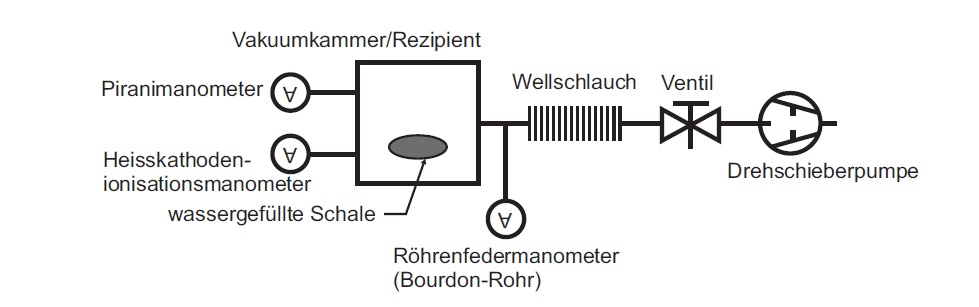
\includegraphics[width=100mm]{Dampf}
	\centering
	\caption{\itshape Blockschaltbild zum Abpumpen kondensierbarer Dämpfe}
	\label{fig:1}
\end{figure}
\noindent

\subsection{Molekular-und Turbomolekularpumpe}
%Hier 2.3, Funktionsweise TMP, mit Gaedestufe, siehe TMP Herstellerangaben hier, kannst einfach die in Anleitung gefragten Werte sonst abschreiben
\begin{figure}[h]
	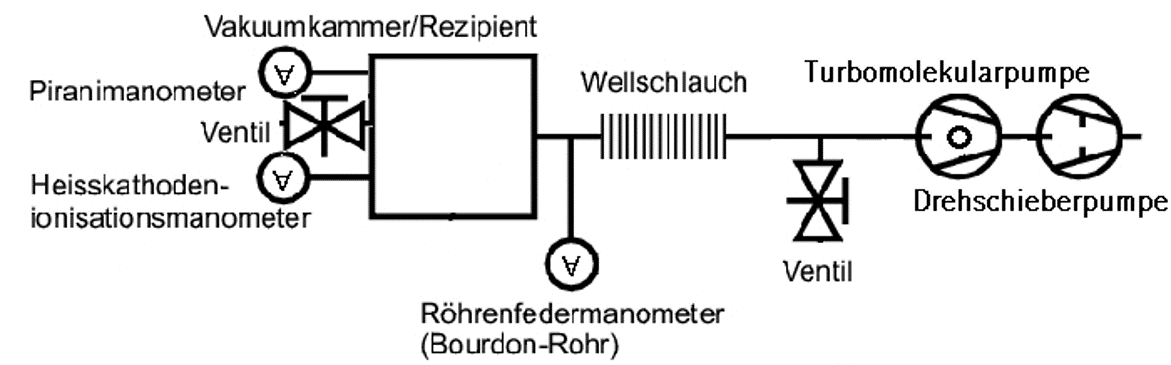
\includegraphics[width=100mm]{TMPmitVorpumpe}
	\centering
	\caption{\itshape Blockschaltbild der Turbomolekularpumpe mit Drehschieberpumpe als Vorpumpe}
	\label{fig:2}
\end{figure}
\noindent

\subsection{Saugvermögen der TMP}
%Hier 2.4, 

\begin{figure}[h]
	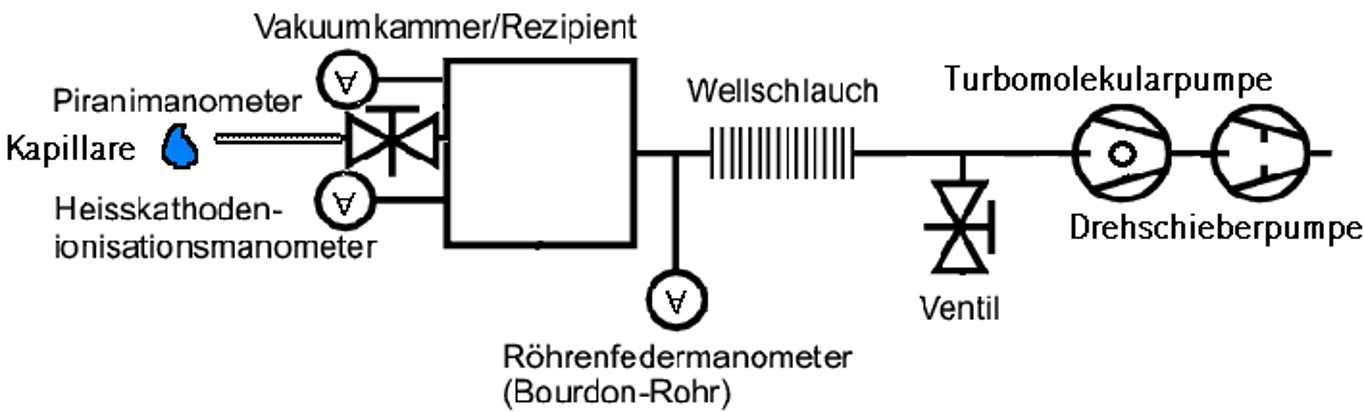
\includegraphics[width=100mm]{Saug}
	\centering
	\caption{\itshape Blockschaltbild Saugvermögen der TMP}
	\label{fig:3}
\end{figure}
\noindent


%\begin{figure}[h]
%	\includegraphics[width=100mm]{SaugvermögenDruck}
%	\centering
%	\caption{\itshape Saugvermögen als Funktion des Logarithmus des Drucks}
%	\label{fig:4}
%\end{figure}
\noindent
\newpage
\subsection{Leitwert von Rohr und Blende}
%Hier 2.5

\begin{figure}[h]
	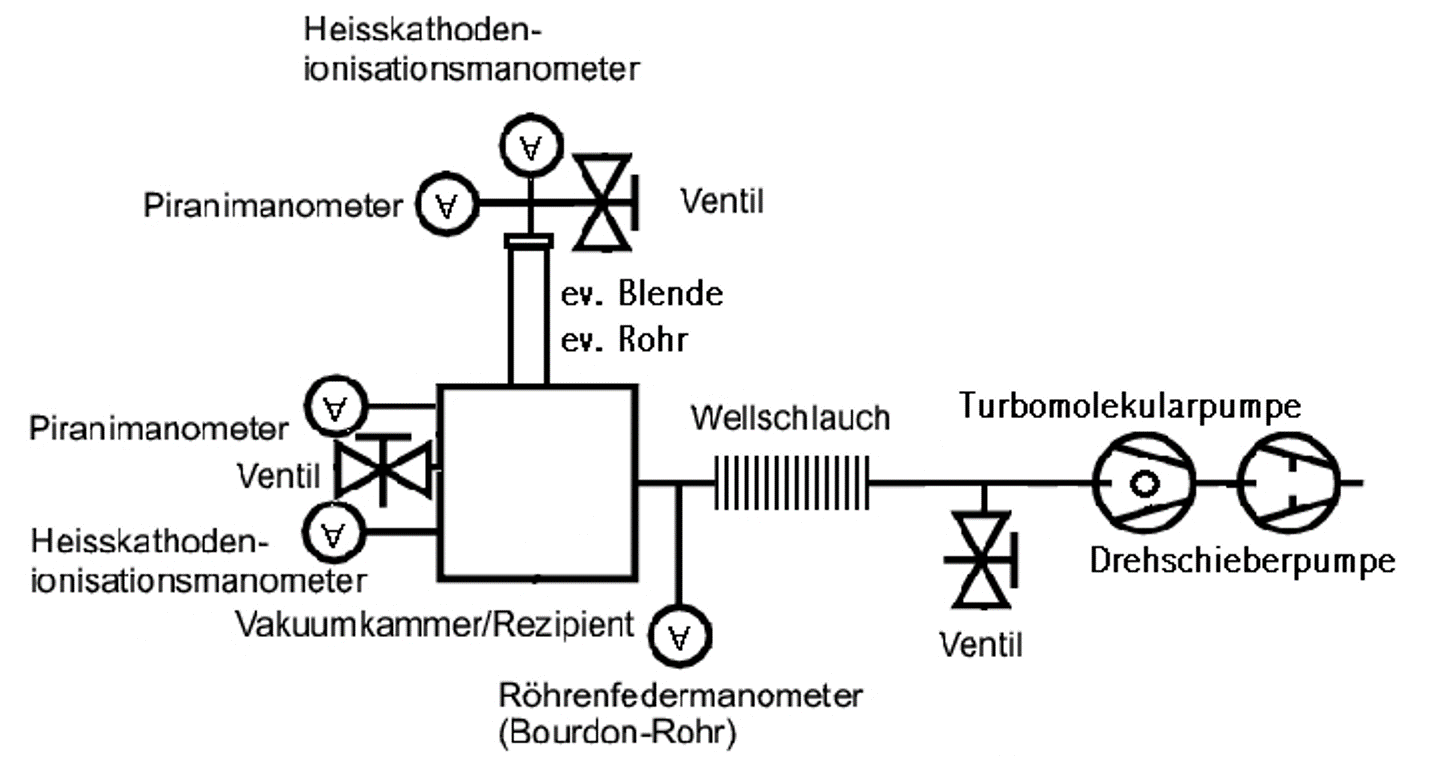
\includegraphics[width=100mm]{LeitwertVonRohrUndBlende}
	\centering
	\caption{\itshape Blockschaltbild Saugvermögen der TMP}
	\label{fig:5}
\end{figure}

%\begin{figure}[h]
%	\includegraphics[width=100mm]{Leitwer1}
%	\centering
%	\caption{\itshape Leitwert von als Funktion des Logarithmus des Drucks}
%	\label{fig:6}
%\end{figure}
\noindent


%\begin{figure}[h]
%	\includegraphics[width=100mm]{Leitwert2}
%	\centering
%	\caption{\itshape Leitwert von als Funktion des Logarithmus des Drucks}
%	\label{fig:7}
%\end{figure}
\noindent



\subsection{Lecksuche}
%Hier 2.6

\begin{figure}[h]
	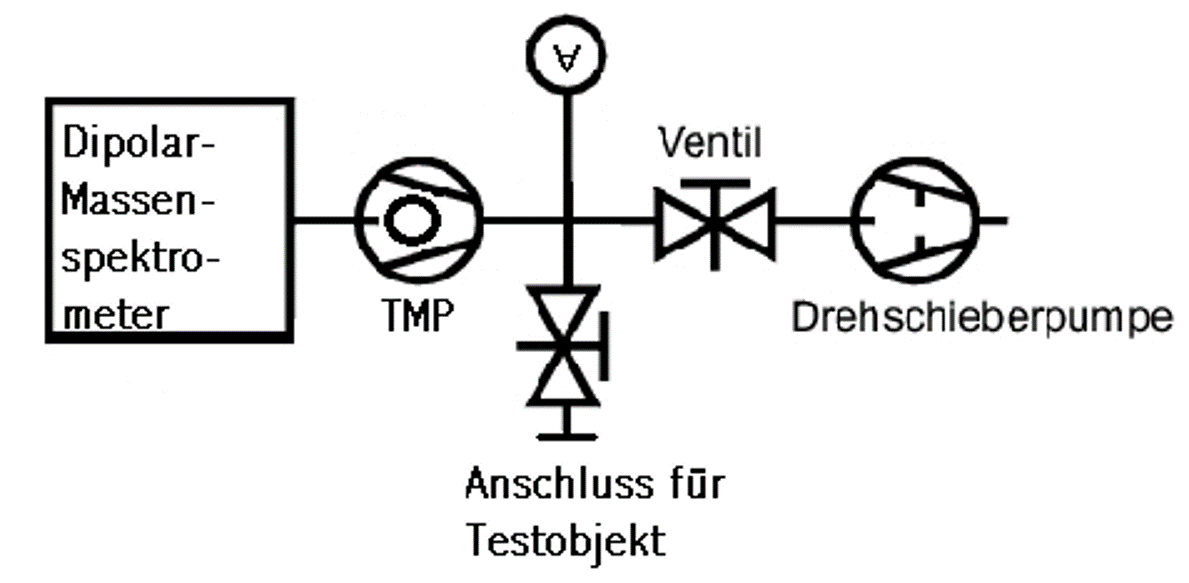
\includegraphics[width=100mm]{GegenstromLecksuche}
	\centering
	\caption{\itshape Blockschaltbild Lecksuche}
	\label{fig:8}
\end{figure}

	\section{Diskussion}

	%\printbibliography
	
	
	
	\begin{thebibliography}{9}
		\bibitem{manual} 
		F13 - Measurement of Muon Properties in the Advanced Students Laboratory. Url: \\\texttt{https://www.physi.uni-heidelberg.de/Einrichtungen/FP/anleitungen/F13.pdf}
		
		\bibitem{particle} 
	     Particle Data Group, Particle data booklet (2008)
		\\\texttt{http://pdg.lbl.gov}
	\end{thebibliography}
	
	
\end{document}